\documentclass[a4paper]{beamer}
\usepackage{fontspec}
%\usepackage[utf8]{inputenc}
\usepackage[english]{babel}
\setsansfont{Calibri}
\setmonofont{Consolas}

\usepackage{minted}

% set default theme
\usetheme{default}

% disable navigation symbols
\setbeamertemplate{navigation symbols}{}

% define greyish background colour for the highlighted code
\definecolor{bg}{rgb}{0.95,0.95,0.95}


\begin{document}

% define title, author and date
\title{Brain Hacking Presentation\\(not to be confused with Chicken, chicken chicken \ldots  chicken) \footnote{\url{https://isotropic.org/papers/chicken.pdf}}}
\author{@SteveClement}
\date{November 8, 2015}


% 1
\frame{\titlepage}

% 2
\begin{frame}
\frametitle{whoami}
steve, hacker, fool, psychonaut, Mensch
\end{frame}

% 3
\begin{frame}
\frametitle{Psychonaut quo vadis?}
In a nutshell: A person navigating his own psyche with different stimuli, IMHO aka. Brain Hacker
\end{frame}

% 4
\begin{frame}
\frametitle{What is Brain Hacking according to Google?}

Googling for Brain Hacking gives 3 interesting top matches:

1. Mind Hacks

2. Neurohacking

3. Mind Performance Hacks

All three on WikiPedia
\\
Brain Hacking will henceforth be referred to as {\bf BH}
\end{frame}

% 5
\begin{frame}
\frametitle{What is Brain Hacking?}
Neurohacking is the colloquial term for (usually personal or "DIY") neuroengineering. It is a form of biohacking (qv) focusing on the brain and CNS. Strictly speaking it is any method of manipulating or interfering with the structure and/or function of neurons for improvement or repair.
\\
Henceforth referred to as {\bf BH}
\end{frame}

% 6
\begin{frame}
\frametitle{What is BH in RL}
\begin{center}
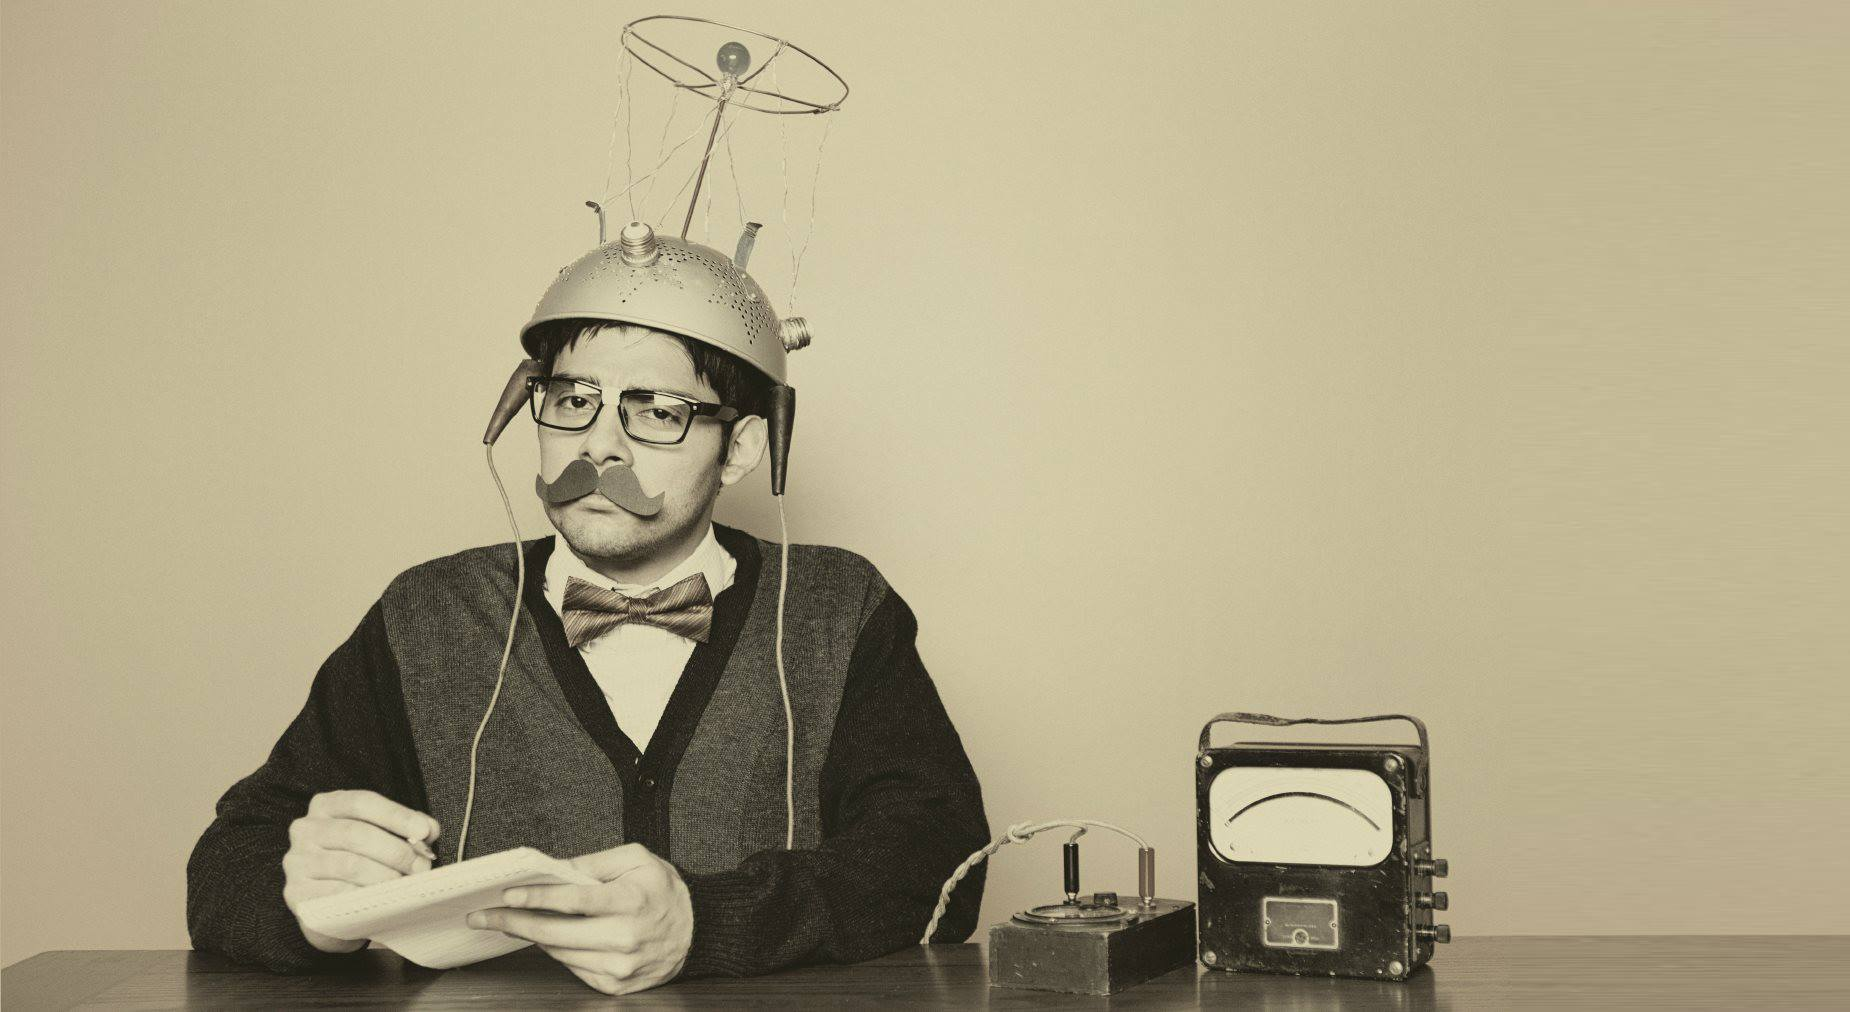
\includegraphics[scale=0.20]{img/mindreader3.jpg}
\end{center}
\end{frame}

% 7
\begin{frame}
\frametitle{Drugs are bad Mkay?}
\being{center}
\includegraphics[scale=0.20]{img/drugsarebad.jpg}
\end{center}
\end{frame}

% 8
\begin{frame}
\frametitle{Drugs are bad according to the state and media?}
Changing paradigm \ldots finally the war on drugs is being seen what it really is and was (a big fuck-off shout-out to the Nixon administration)
% Universal text on drugs, doesn't even mention what a drug is, c.f  Lobbying and the problems it would generate for the legal drugs
\end{frame}

% 9
\begin{frame}
\frametitle{Media disinformation}
\being{center}
\includegraphics[scale=0.20]{img/disinformation.jpg}
\end{center}
% Winehouse example, MDMA Holes in the brain example
\end{frame}

% 10
\begin{frame}
\frametitle{Media Political spectrum}
% Right wing vs. Left wing vs. other types
\end{frame}

% 11
\begin{frame}
\frametitle{Why o' Why?}
% Lobby, legal drug market, big pharma, big tobacco, big "beer"
\end{frame}

% 12
\begin{frame}
\frametitle{Drugs are not that bad according to the state and media!}
Changing paradigm \ldots finally, everything is a drug not everything is a bad drug.
% Dosage
\end{frame}

% 13
\begin{frame}
\frametitle{How?}
\end{frame}

% 14
\begin{frame}
\frametitle{How?}
\inputminted[firstline=1, lastline=6, gobble=0, linenos, mathescape, bgcolor=bg, numbersep=8pt, frame=lines, framesep=3mm, fontsize=\scriptsize]{python}{code/bh.py}
\end{frame}

% 15
\begin{frame}
\frametitle{Demo with lea and the actual generator}
Goo does not play dice
\\

\includegraphics[scale=0.60]{img/mjr_anarchist_flag.jpg}
\\
(Anarcho Syndicalism, Google it and become an atheist nihilist)
\end{frame}

% 16
\begin{frame}
\frametitle{SO sorry\ldots}
I broke some laws, mostly copyright laws.
\\
Credit where credit is due, all my sources are amazing people. Thanks.
\end{frame}

% 17
\begin{frame}
\frametitle{Thanks for the fish and do not believe the hype}
\begin{center}
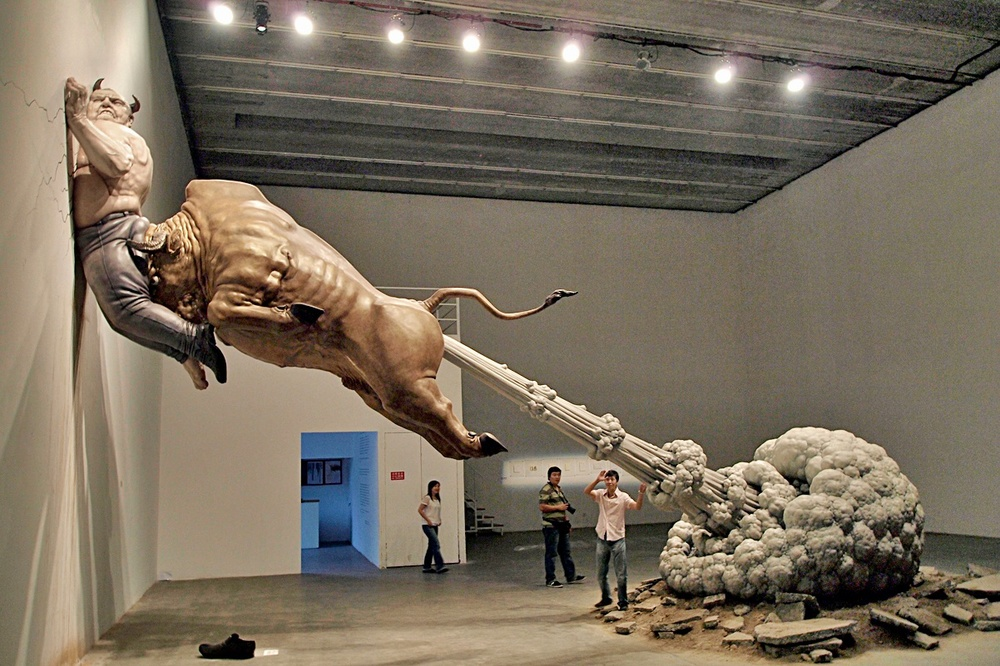
\includegraphics[scale=1.00]{img/bullshit-sculpture.jpg}
\end{center}
Created in \LaTeX{} with 
\includegraphics[scale=0.05]{img/polyamory.png}
\end{frame}

\end{document}